\subsection{Need for an integrated modeling pipeline}

The overarching objective of this project is to develop an integrated modeling pipeline that encompasses land use, travel demand and traffic assignment to model the combined and cumulative impacts of transportation infrastructure and land use regulations. A key motivation for developing such a model system is that the urban environment
is complex enough that it is not feasible to anticipate the effects of alternative infrastructure investments and land use policies without some form of analysis that could reflect the cause and effect interactions that could have both intended and unintended consequences.

Consider a highway expansion project, for example. Traditional civil engineering training from the mid 20\textsuperscript{th} century suggested that the problem was a relatively simple one: excess demand meant that vehicles were forced to slow down, leading to congestion bottlenecks. The remedy was seen as easing the bottleneck by adding capacity, thus restoring the balance of capacity to demand. Unfortunately, as Downs (2004) has articulately explained, and most of us have directly observed, once capacity is added it is quickly used, leading some to conclude that \enquote{you can't build your way out of congestion}.

Highway congestion is a difficult problem because individuals and organizations adapt to changing circumstances. When new capacity is available vehicle speeds initially increase, but this drop in travel time on the highway allows drivers taking other routes to change to this now-faster route, or to change their commute to work from a less-convenient shoulder of the peak time to a mid-peak time, or to switch from transit or car-pooling to driving alone, adding demand at the most desired time of the day. Over the long-term, developers take advantage of the added capacity to build new housing and commercial and office space, households and firms take advantage of the accessibility to move farther out where sites are less expensive.

The highway expansion example illustrates a broader theme: urban systems, including the transportation network, the housing market, the labor market (commuting), and other real estate markets are closely interconnected, much like the global financial system. An action taken in one sector ripples through the entire system to varying degrees, depending on how large the intervention is and what other interventions are occurring at the same time.

This brings us to a second broad theme: interventions are rarely coordinated with each other, and often are conflicting or have a compounding effect that was not intended. This pattern is especially true in metropolitan areas consisting of many local cities and possibly multiple counties - each of which retain control of land use policies over a fraction of the metropolitan area, and none of which have a strong incentive, nor generally the means, to coordinate their actions. It is often the case that local jurisdictions are taking actions in strategic ways that will enhance their competitive position for attracting tax base-enhancing development and residents. It is also systematically the case that transportation investments are evaluated independently of land use plans and the reactions of the real estate market.

In order to better support the analysis of the impacts of transportation infrastructure and land use regulations within large and complex urban regions, we propose to develop an integrated pipeline for modeling urban land use, travel demand and traffic assignment and to compute transportation-related energy consumption. The project lends itself to further extension to address building energy consumption as well, providing a potential to coherently simulate transport and building energy demand for the first time in a coherent way, at an urban and metropolitan scale. 


\subsection{Overview of pipeline architecture}

Three models are integrated within this project. UrbanSim is an open source model system developed to represent long-term dynamics of urban development and its interaction with transportation systems. ActivitySim is an activity-based travel demand model system, and it was developed using the UrbanSim platform as its starting point. The third model component is a static user equilibrium traffic assignment model using a standard Frank-Wolfe algorithm.

\begin{figure}[htbp]
  \center
  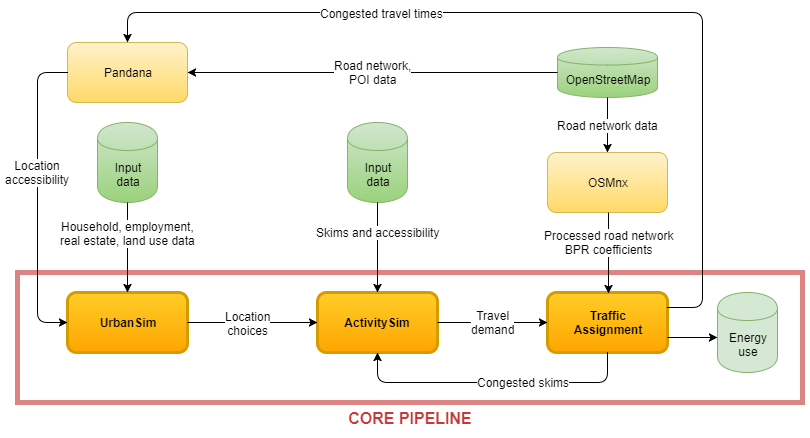
\includegraphics[width=\textwidth]
  {graphics/diagram_pipeline.png}
  \caption{Overview of the integrated modeling pipeline's architecture}
  \label{fig:overview_pipeline_architecture}
\end{figure}

While UrbanSim and ActivitySim are microsimulation models, meaning that they operate at the level of individuals and households, the traffic assignment model is an aggregate traffic flow model that has been parallelized in a high-performance computing (HPC) environment. Figure \ref{fig:overview_pipeline_architecture} depicts the proposed pipeline for integrating these three models.
